\documentclass[border=15pt, multi, tikz]{article}
\usepackage[backend=bibtex,style=authoryear,natbib=true]{biblatex} % Use the bibtex backend with the authoryear citation style (which resembles APA)

\addbibresource{example.bib} % The filename of the bibliography

\usepackage[autostyle=true]{csquotes} % Required to generate language-dependent quotes in the bibliography
\usepackage{import}
\usepackage{tikz}
\usepackage{tikz-network}
\usetikzlibrary{calc,patterns,angles,quotes}
\usepackage{breqn}
\usepackage{bm}
\usepackage{float}
\usepackage{graphicx}
\usepackage{subcaption}
\usepackage{multirow}
\usepackage{graphicx}
\usepackage{rotating}
\usepackage{booktabs}
\usetikzlibrary{fit}
\usetikzlibrary {arrows.meta,graphs,shapes.misc}
\usetikzlibrary {positioning}
\subimport{./layers/}{init}
\newcommand{\bn}{\textbf{n}}
\newcommand{\tabhead}[1]{\textbf{#1}}

\def\ConvColor{rgb:yellow,5;red,2.5;white,5}
\def\ConvReluColor{rgb:yellow,5;red,5;white,5}
\def\PoolColor{rgb:red,1;black,0.3}
\def\DcnvColor{rgb:blue,5;green,2.5;white,5}
\def\SoftmaxColor{rgb:magenta,5;black,7}
\def\SumColor{rgb:blue,5;green,15}
\def\poolsep{1}


\begin{document}


\section{Training Details}

The models are trained on dataset "synthetic-50-5" as mentioned in Chapter \ref{ch:04} with 3000 scenes. Each scene has a depth map with dimension $ 128\times 128 $ in height and width, an image with dimension $ 128\times 128 \times 1 $.  The depth map is converted to 3D vertex map as introduced in Chapter \ref{ch:04}. The light map is calculated based on vertex map and the known light position. We create a tensor in PyTorch that includes vertex map, image and the light direction for each scene and considered it as one training case. Thus 3000 scenes has corresponding 3000 training cases. Each scene has a corresponding ground-truth normal map for loss calculation and the evaluation. 

\begin{figure}[H]
	\centering
	
	\begin{subfigure}[b]{0.24\linewidth}
		
\includegraphics[width=\linewidth]{./Figures/test_scenes/03094.depth0.png}
	\end{subfigure}
	\begin{subfigure}[b]{0.24\linewidth}
		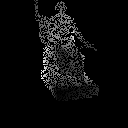
\includegraphics[width=\linewidth]{./Figures/test_scenes/03094.depth0_noise.png}
	\end{subfigure}
	\begin{subfigure}[b]{0.24\linewidth}
		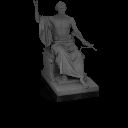
\includegraphics[width=\linewidth]{./Figures/test_scenes/03094.image0.png}
	\end{subfigure}
	\begin{subfigure}[b]{0.24\linewidth}
		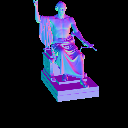
\includegraphics[width=\linewidth]{./Figures/test_scenes/03094.normal0.png}
	\end{subfigure}
	

	\begin{subfigure}[b]{0.24\linewidth}
		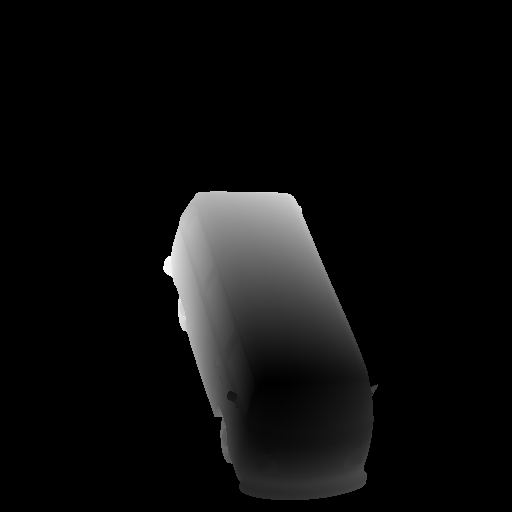
\includegraphics[width=\linewidth]{./Figures/test_scenes/05126.depth0.png}
		\caption{Depth Map}
	\end{subfigure}
	\begin{subfigure}[b]{0.24\linewidth}
		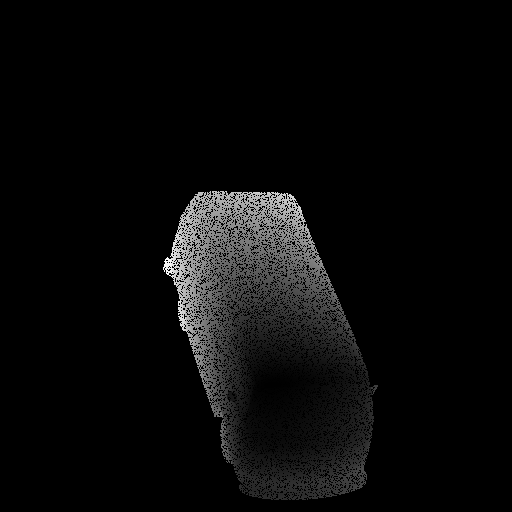
\includegraphics[width=\linewidth]{./Figures/test_scenes/05126.depth0_noise.png}
		\caption{Add noise}
	\end{subfigure}
	\begin{subfigure}[b]{0.24\linewidth}
		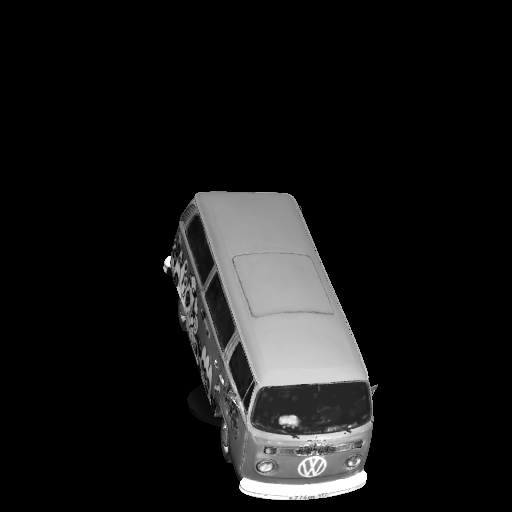
\includegraphics[width=\linewidth]{./Figures/test_scenes/05126.image0.png}
		\caption{Image}
	\end{subfigure}
	\begin{subfigure}[b]{0.24\linewidth}
		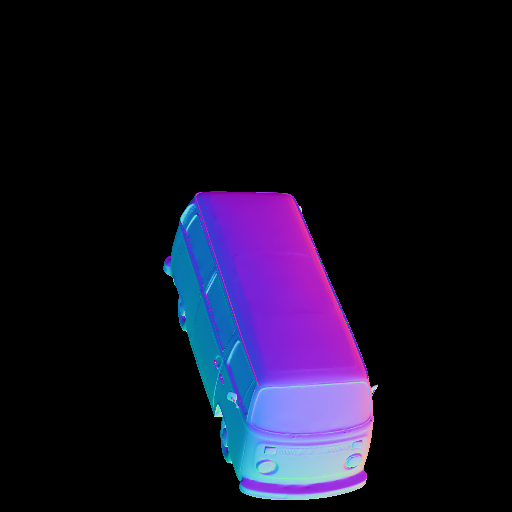
\includegraphics[width=\linewidth]{./Figures/test_scenes/05126.normal0.png}
		\caption{Normal}
	\end{subfigure}
	
	\caption{Some of the test scenes during the training. From top to bottom, baoshanlu, Washington, Garfield, Dragon, Bus}
	\label{fig:test-scene}
\end{figure}


The training processes are evaluated in every epochs with 29 evaluation scenes that models never seen before, which contains the 5 different objects in the ``synthetic-50-5" test set. Figure \ref{fig:test-scene} shows some of the test scenes during the training work. Note that the position of objects are not placed always naturally on the stage but with a random rotation in X, Y, Z axes, respectively.

For the training parameters, we set the training pipeline with batch size $ 8 $, we found that a higher batch size will reduce the final performance.  Adam optimizer (\cite{adam}), learning rate start from  $ 1\times10^{-3} $, learning schedule [8,1000], learning decay factor 0.5. The model is trained with PyTorch 1.10.0a0, CUDA 11.4.1, GPU with single NVIDIA GEFORCE RTX 3090. It takes 14 hours to train GCNN and 35 hours to train the Trip-Net. We terminate the training when the evaluation on the test dataset converged.


\section{GCNN model based on Geometry Information}
The GCNN model is the base model of the whole thesis. The architecture is described in \ref{sec:gcnn}. We use a single GCNN to estimate the surface normal based on geometry information. It uses vertex map as input to estimate the corresponding tangent surface normal map. 


\begin{figure}[H]
	\centering
	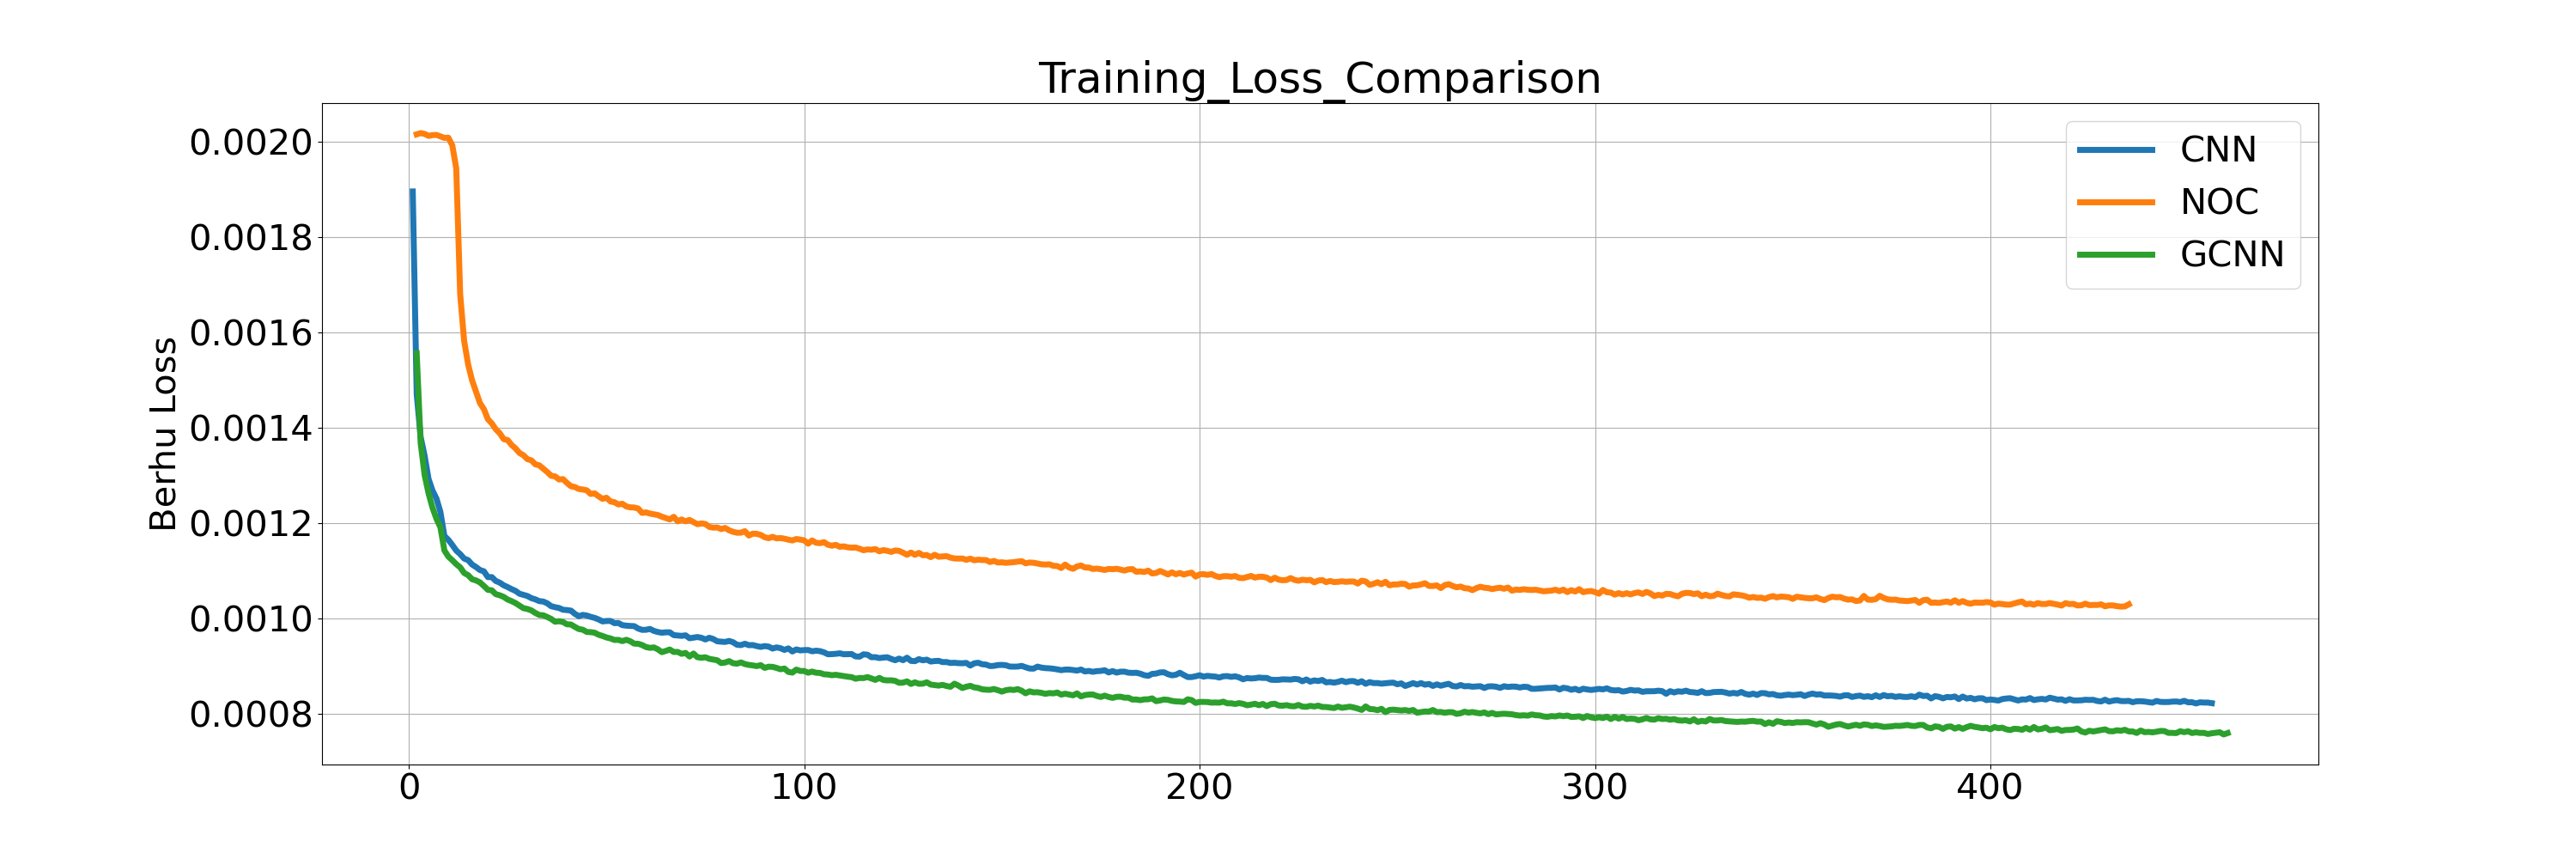
\includegraphics[width=\textwidth]{./Figures/gcnn_training_loss.png}
	
	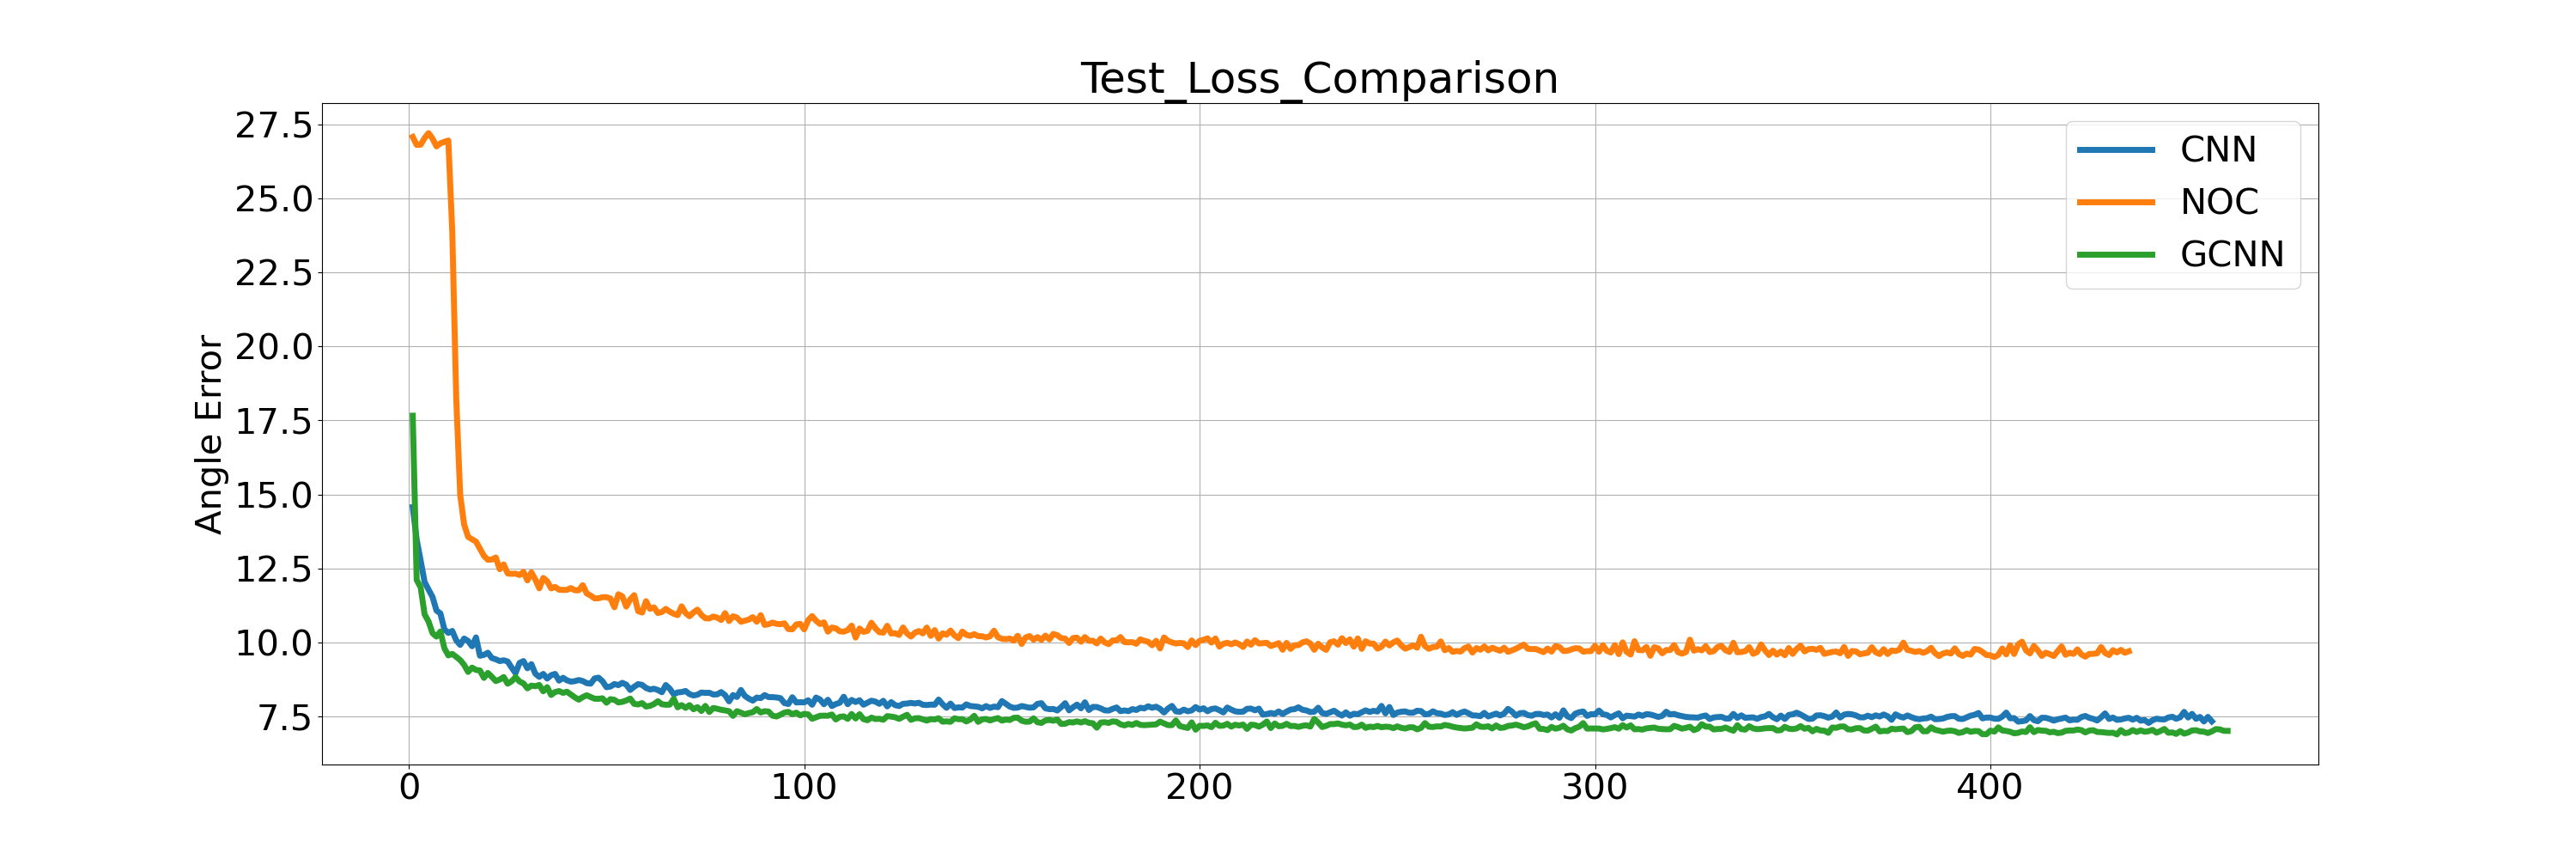
\includegraphics[width=\textwidth]{./Figures/gcnn_eval_loss.png}
	\caption{The training history of GCNN model. The line chart records the training BerHu loss of the model GCNN, NOC and CNN. The left shows the training loss history whereas the right one shows the evaluation loss history.}
	\label{fig:gcnn-training-history}
\end{figure}

In order to verify the applicability of the skip connection and the gated convolution layers, we trained two extra models as a comparison. The first model, we replace all of the gated layer to standard convolution layers in the network but keeps all of the other settings same, and give it a name ``CNN". It is used to verify the performance the gated convolution layers. As mentioned in chapter \ref{ch:03}, the gated layer is designed to deal with noised input. Since all of the vertex map in the dataset has been added noise, the GCNN is supposed to over-perform ``CNN". 
Another model called ``NOC" is designed to verify the skip connection, which simply removes the skip connections in the network but keeps other settings same. Is is designed to show to which content will skip connection help the model performance. We use Reversed Huber Loss as loss function during the training, since we found it gives a better final error compare to L2 loss. The model is evaluated after every epoch training and calculate the angle error on the test dataset. The training history is shown in Figure \ref{fig:gcnn-training-history}. 


%% TODO
waiting for the experiment, then describe the chart...


\begin{table}[H]
	
	\centering
	\begin{tabular}{l l l l l l }
		\tabhead{Model} & $ \# $\textbf{Total} &\textbf{ V-P} & \textbf{L-P} & \textbf{I-P} & \tabhead{Size /MB}\\
		\hline
		CNN 					& 17 & 32 & 0 & 0 & 25.5 \\
		\hline
		NOC 					& 32 & 32 & 0 & 0 & 30.6 \\
		\hline
		GCNN 					& 32 & 32 & 0 & 0 & 45.8 \\
	\end{tabular}
	\caption{GCNN Model information. Columns V-P, L-P and I-P represent the number of convolution layers in vertex pipe, light pipe and image pipe respectively. Note that one gated convolution layer is constructed with 2 standard layers, thus it is counted as 2. }	
	\label{tab:gcnn-eval-mean}
\end{table}




\section{Trip-Net model based on Calibrated Illuminated RGB-D Image}
The Trip-Net model uses three times GCNN architecture with 4 times fusions, which is more difficult to train. It takes the calibrated illuminated RGB-D images as input to estimate the surface normal map. When we train this model, we take the GCNN model as a baseline, to observe the beneficial of illuminated information using with Trip-Net architecture.
 Since it is more complicate than GCNN, we also explored the optimum fusion times of the Trip-Net to see any possibility for the model simplification. A set of similar models have been trained with same settings but different fusion times, denotes by Trip-Net-F$ x $, where $ x $ denotes the fusion times. We evaluate the fusion times from 1 to 4. For the learning rate.  we set $ 1e-3 $. It goes well with GCNN model but lead to loss explosion in Trip-Net. Thus we set a learning rate schedule with an extra decay step at epoch 8. The decay factor is $ 0.5$. The batch size is chosen as 8.

Figure \ref{fig:trip-net-training-history} shows the training history of Trip-Net models on BerHu Loss. As shown in the loss figure, all of the four models has a reasonable learning rate. 
From the chart we can see that, trip-Net with four times fusion converges obviously faster than fewer fusion times model. However, model F3 with 3 times fusion converge slower than F4 but in the end it achieves a similar evaluation loss with F4. The F1 and F2 models are relatively weaker than the other two models. 


\begin{figure}[H]
	\centering
	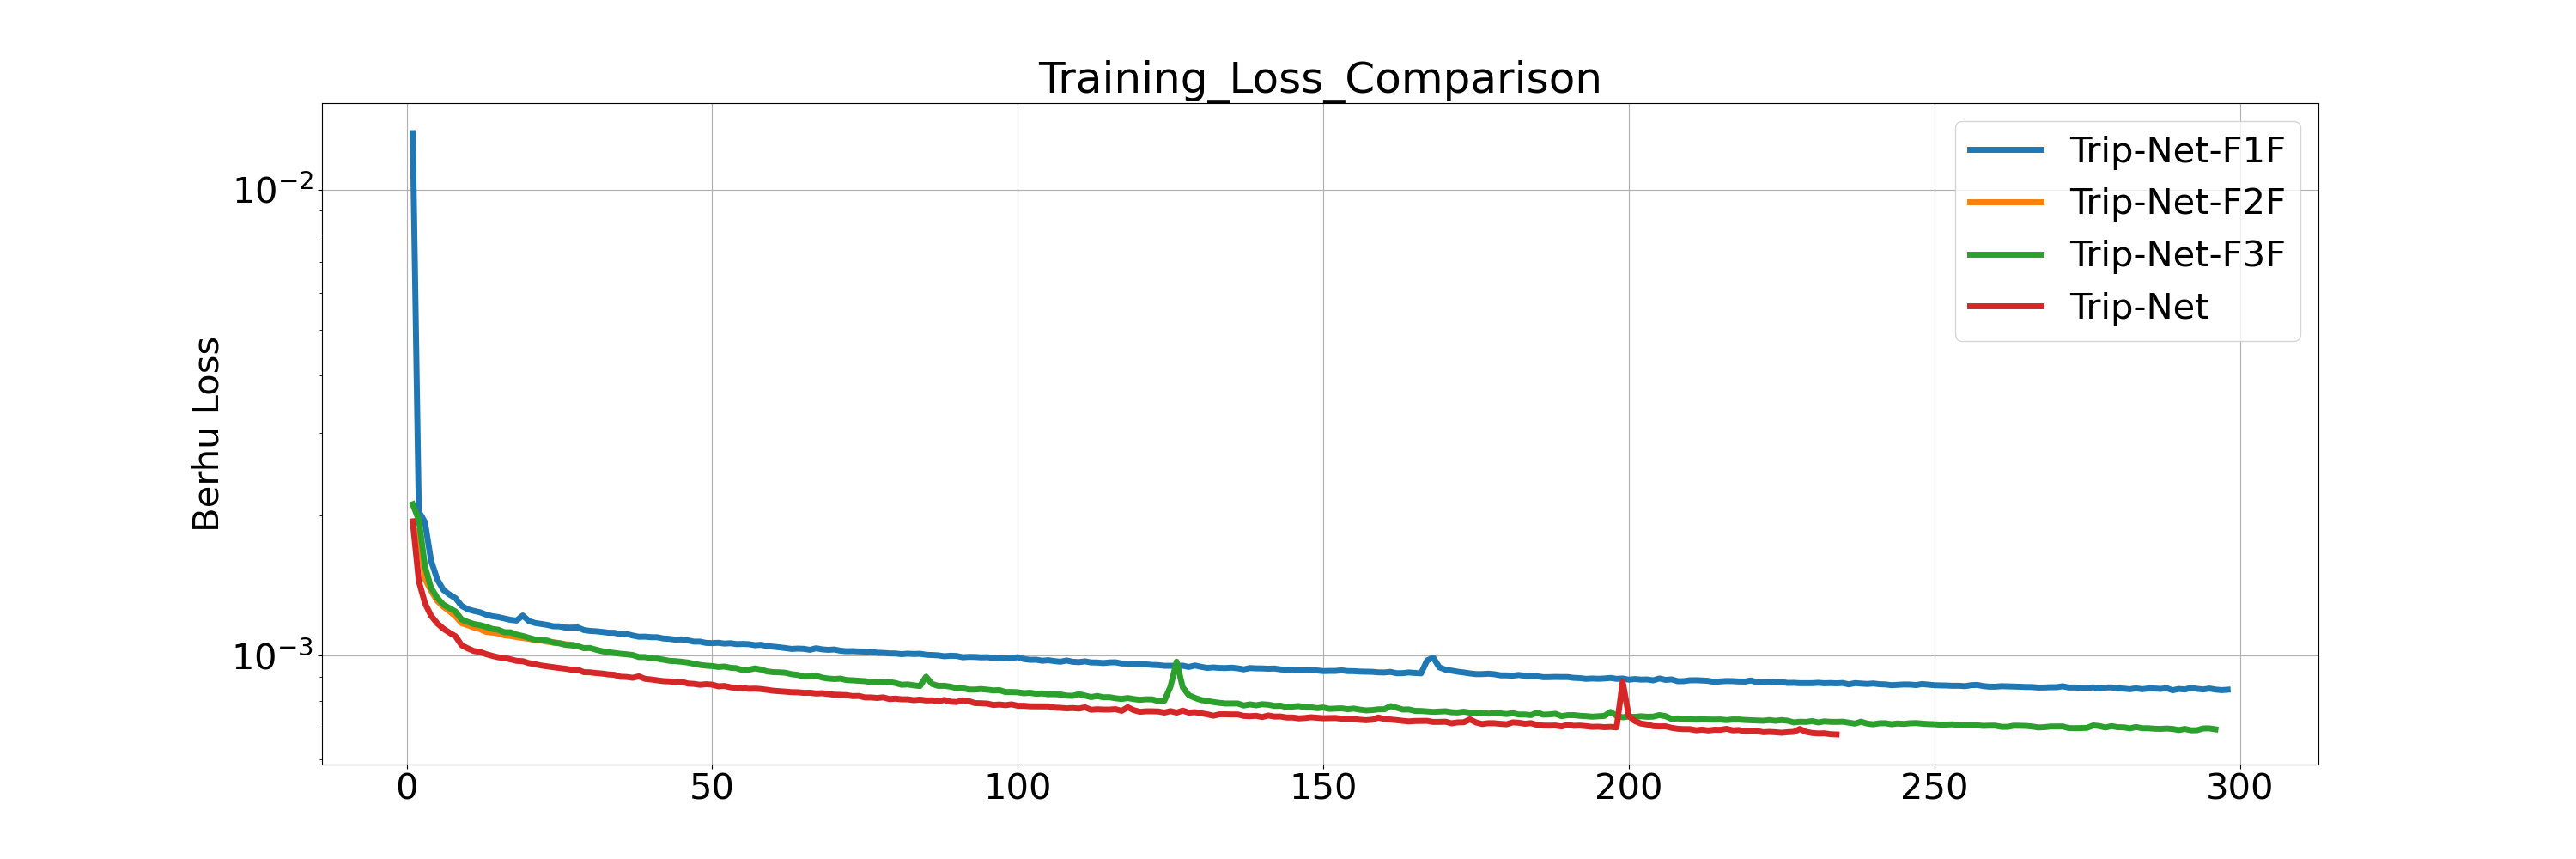
\includegraphics[width=\textwidth]{./Figures/trip_net_training_loss.png}
	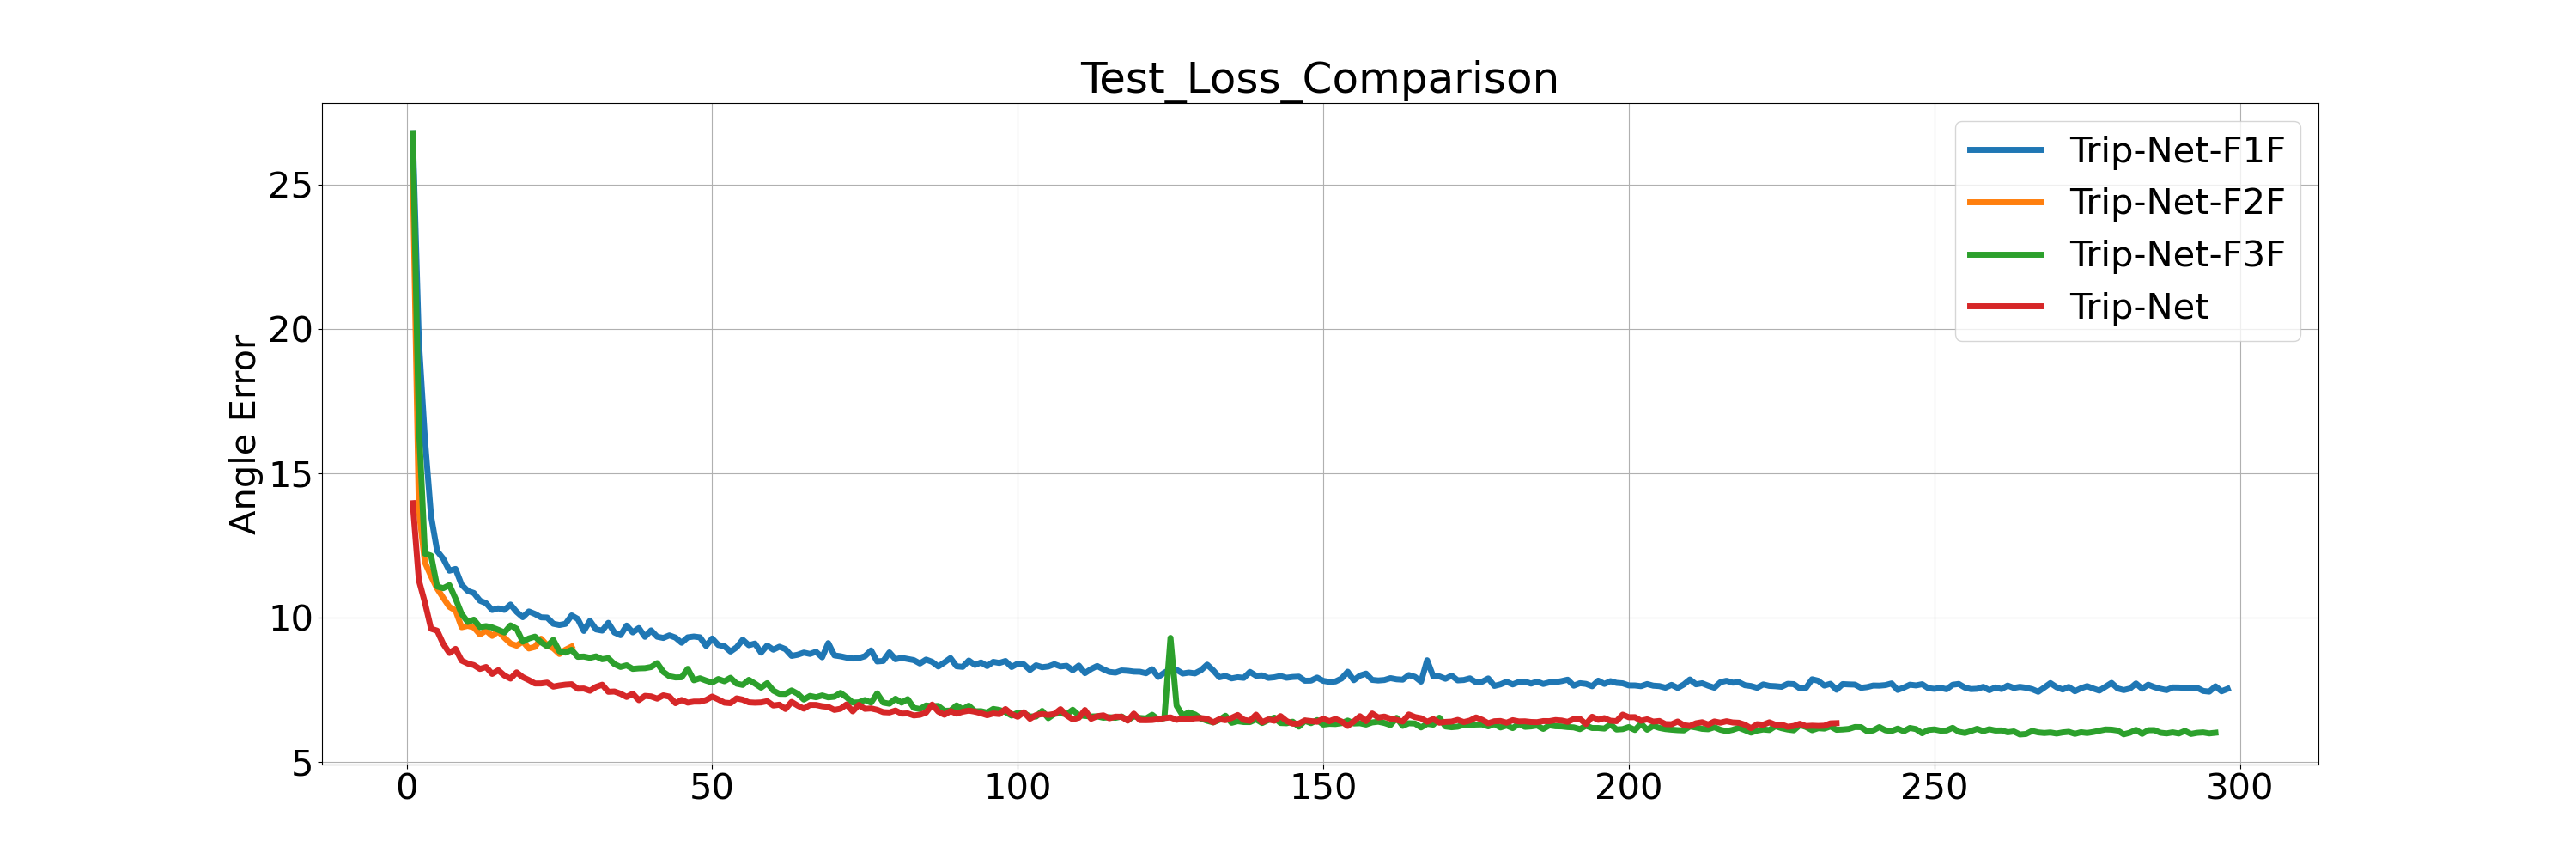
\includegraphics[width=\textwidth]{./Figures/trip_net_eval_loss.png}
	\caption{The training history of Trip-Net model. The line chart records the training BerHu loss of the model Trip-Net, Trip-Net-F1, Trip-Net-F2, Trip-Net-F3, GCNN.}
	\label{fig:trip-net-training-history}
\end{figure}


However, the sacrifice of accuracy gives a relatively lighter model. Since we remove the fusions between different pipes, the corresponding upsampling layers in the image and light pipes can also be removed. The model can be trained faster and the size is reduced as well. Table \ref{tab:trip-net-size-compare} gives a comparison of the size and training time among different models.


\begin{table}[H]
	
	\centering
	\begin{tabular}{l l l l l l l }
		\tabhead{Model} & $ \# $\textbf{Total} &\textbf{ V-P} & \textbf{L-P} & \textbf{I-P} & \tabhead{Size /MB} & \tabhead{Time /h}\\
		Trip-Net-F1F  			& 88 &  40 & 24 & 24 & 106  &  9.82\\ 
		\hline
		Trip-Net-F2F 			& 92 & 40 & 26 & 26 & 137 &  7.35\\ 
		\hline
		Trip-Net-F3F 			& 96 & 40 & 28 & 28 & 167 &  7.35\\
		\hline
		Trip-Net 				& 100 & 40 & 30 & 30 & 198 & 9.15\\
	\end{tabular}
	\caption{Trip-Net Model information. Columns V-P, L-P and I-P represent the number of convolution layers in vertex pipe, light pipe and image pipe respectively. Note that one gated convolution layer is constructed with 2 standard layers, thus it is counted as 2. }	
	\label{tab:trip-net-size-compare}
\end{table}


\section{Quantitative Evaluation}

Based on metrics proposed by \cite{geometry_based_solution}, 6 different metrics are used for evaluation. Note that the input vertex map is only semi-dense. One of the benefit of GCNN architecture is the robust to the noisy input, thus in the evaluation, all the points including missing points in the input vertex map are taken into account. 

\paragraph{Average Angle Error Metric}
The metric calculate the average angle error for each point between the inferred normal and ground-truth normal. 
\paragraph{Median Angle Error Metric}
The metric calculate the median angle error of all the point in the normal map.
\paragraph{5 Degree Error Metric}
The metric calculate the percentage of the predicted normals that has error less than 5 degrees comparing to ground-truth.
\paragraph{11.5 Degree Error Metric}
The metric calculate the percentage of the predicted normals that has error less than 11.5 degrees comparing to ground-truth.
\paragraph{22.5 Degree Error Metric}
The metric calculate the percentage of the predicted normals that has error less than 22.5 degrees comparing to ground-truth.
\paragraph{30 Degree Error Metric}
The metric calculate the percentage of the predicted normals that has error less than 30 degrees comparing to ground-truth.

We evaluate the trained models on ``synthetic-50-5". 5 objects are considered in the test dataset. They are: $ Baoshanlu $, $ Bus $, $ Dragon $, $ Garfield $, and $ Washington $. Each object has 20 scenes with total 100 scenes for 5 objects. The test objects do not exist in the training dataset. We evaluate all the presented models on the test dataset, in order to fit them in one table, the name of each models are simplified. $ SVD $ model use SVD optimization method, $ NOC $ model is the no skip connection version of $ GCNN $, $ CNN $ is the CNN version of $ GCNN $. $ F1 $, $ F2 $, $ F3 $,$ F4 $ means the fusion times in the Trip-Net. 

Among all the columns, the most important models are $ GCNN $ (depth map based) and  $ F4 $ (calibrated illuminated RGB-D image based), which is the core result of this thesis. When evaluate the $ GCNN $ models, we can take $ SVD $ model as baseline, $ NOC $ and $ CNN $ are used to verify the performance of $ GCNN $ model. When evaluate the $ F1-F4 $ models, we can take $ GCNN $ model as baseline.


%% mean metric
\begin{table}[H]
	\centering
	\begin{tabular}{l l | l | l l l | l l l l }
		\tabhead{Object} & $ \# $ & \tabhead{SVD} & \tabhead{GCNN} & \tabhead{NOC} & \tabhead{CNN} & \tabhead{F1}& \tabhead{F2}& \tabhead{F3}& \tabhead{F4}\\
		Baoshanlu  		& 20 & 35.66 & 11.09 & 13.58 & 15.55 & 11.22 & 10.36 & & 9.82 \\ 
		\hline
		Bus 			& 20 & 31.93 & 7.79 & 8.95 & 11.93 & 7.49 & 7.85 & & 7.32\\ 
		\hline
		Dragon 			& 20 & 39.57 & 10.60 & 15.29 & 16.03 & 10.47 & 10.23 & & 7.35 \\
		\hline
		Garfield 		& 20 & 39.69 & 10.20 & 12.50 & 14.46 & 9.94 & 10.36 & & 9.15 \\
		\hline
		Washington 		& 20 & 42.83 & 13.43 & 17.59 & 18.71 & 13.32 & 13.40 & & 12.13\\
	\end{tabular}
	\caption{Average Angle Error of the evaluation dataset.}	
	\label{tab:eval-mean}
\end{table}

%% median metric
\begin{table}[H]
	\centering
	\begin{tabular}{l l | l | l l l | l l l l }
		\tabhead{Object} & $ \# $ & \tabhead{SVD} & \tabhead{GCNN} & \tabhead{NOC} & \tabhead{CNN} & \tabhead{F1}& \tabhead{F2}& \tabhead{F3}& \tabhead{F4}\\
		Baoshanlu  		& 20 & 34.06 & 8.86 & 10.82 & 13.25 & 8.95 & 8.02 & & 7.62 \\ 
		\hline
		Bus 			& 20 & 34.14 & 4.44 & 5.02 & 8.69 & 4.11 & 4.58 & & 4.01 \\ 
		\hline
		Dragon 			& 20 & 36.43 & 7.62 & 11.10 & 13.26 & 7.60 & 7.12 & & 5.06 \\
		\hline
		Garfield 		& 20 & 37.60 & 6.40 & 8.90 &11.31 & 6.30 & 6.72 & & 5.81\\
		\hline
		Washington 		& 20 & 36.89 & 7.64 & 11.38 & 13.64& 7.49 & 7.60 & & 6.76\\
	\end{tabular}
	\caption{Median Angle Error of the evaluation dataset.}	
	\label{tab:eval-median}
\end{table}


%% 5 degree metric
\begin{table}[H]
	\centering
	\begin{tabular}{l l | l | l l l |l l l l }
		\tabhead{Object} & $ \# $ & \tabhead{SVD} & \tabhead{GCNN} & \tabhead{NOC} & \tabhead{CNN} & \tabhead{F1}& \tabhead{F2}& \tabhead{F3}& \tabhead{F4}\\
		Baoshanlu  		& 20 & 0.01 & 0.25 & 0.18 & 0.11 & 0.24 & 0.31 & & 0.31\\ 
		\hline
		Bus 			& 20 & 0.00 & 0.56 & 0.50 & 0.23 & 0.59 & 0.54 & & 0.59 \\ 
		\hline
		Dragon 			& 20 & 0.00 & 0.31 & 0.17 & 0.10 & 0.31 & 0.34 & & 0.50\\
		\hline
		Garfield 		& 20 & 0.00 & 0.41 & 0.27 & 0.14 & 0.42 & 0.39 & & 0.45\\
		\hline
		Washington 		& 20 & 0.00 & 0.38 & 0.26 & 0.10 & 0.36 & 0.36 & & 0.41\\
	\end{tabular}
	\caption{Percent of error less than 5 degree of the evaluation dataset.}	
	\label{tab:eval-5d}
\end{table}


%% 11.5 degree metric
\begin{table}[H]
	\centering
	\begin{tabular}{l l | l | l l l | l l l l }
		\tabhead{Object} & $ \# $ & \tabhead{SVD} & \tabhead{GCNN} & \tabhead{NOC} & \tabhead{CNN} & \tabhead{F1}& \tabhead{F2}& \tabhead{F3}& \tabhead{F4}\\
		Baoshanlu  		& 20 & 0.03 & 0.62 & 0.52 & 0.41 &  0.62 & 0.66 & & 0.69\\ 
		\hline
		Bus 			& 20 & 0.05 & 0.81 & 0.78 & 0.65 & 0.83 & 0.82 & & 0.83 \\ 
		\hline
		Dragon 			& 20 & 0.02 & 0.69 & 0.51 & 0.40 & 0.70 & 0.71 & & 0.82\\
		\hline
		Garfield 		& 20 & 0.03 & 0.72 & 0.62 & 0.51 &0.73 & 0.71  & & 0.75\\
		\hline
		Washington 		& 20 & 0.02 & 0.62 & 0.50 & 0.40 & 0.63 & 0.62 & & 0.66\\
	\end{tabular}
	\caption{Percent of error less than 11.5 degree of the evaluation dataset.}	
	\label{tab:eval-11d}
\end{table}



%% 22.5 degree metric
\begin{table}[H]
	\centering
	\begin{tabular}{l l | l | l l l | l l l l }
		\tabhead{Object} & $ \# $ & \tabhead{SVD} & \tabhead{GCNN} & \tabhead{NOC} & \tabhead{CNN} & \tabhead{F1}& \tabhead{F2}& \tabhead{F3}& \tabhead{F4}\\
		Baoshanlu  		& 20 & 0.18 & 0.90 & 0.84 & 0.79 & 0.90 & 0.91 & & 0.92\\ 
		\hline
		Bus 			& 20 & 0.26 & 0.93 & 0.91 & 0.89 & 0.93 & 0.93 & & 0.94\\ 
		\hline
		Dragon 			& 20 & 0.14 & 0.90 & 0.79 & 0.80 & 0.90 & 0.90 & & 0.95\\
		\hline
		Garfield 		& 20 & 0.13 & 0.89 & 0.86 & 0.84 & 0.90 & 0.89 & & 0.91\\
		\hline
		Washington 		& 20 & 0.14 & 0.81 & 0.72 & 0.72 & 0.81 & 0.81 & & 0.84\\
	\end{tabular}
	\caption{Percent of error less than 22.5 degree of the evaluation dataset.}	
	\label{tab:eval-22d}
\end{table}


%% 30 degree metric
\begin{table}[H]
	\centering
	\begin{tabular}{l l | l | l l l | l l l l }
		\tabhead{Object} & $ \# $ & \tabhead{SVD} & \tabhead{GCNN} & \tabhead{NOC} & \tabhead{CNN} & \tabhead{F1}& \tabhead{F2}& \tabhead{F3}& \tabhead{F4}\\
		Baoshanlu  		& 20 & 0.37 & 0.96 & 0.93 & 0.90 & 0.96 & 0.96 & & 0.97 \\ 
		\hline
		Bus 			& 20 & 0.43 & 0.96 & 0.94 & 0.93 & 0.96 & 0.96 & & 0.96 \\ 
		\hline
		Dragon 			& 20 & 0.30 & 0.95 & 0.88 & 0.90 & 0.95 & 0.95 & & 0.98 \\
		\hline
		Garfield 		& 20 & 0.27 & 0.94 & 0.92 & 0.91 & 0.94 & 0.94 & & 0.95 \\
		\hline
		Washington 		& 20 & 0.28 & 0.88 & 0.81 & 0.82 & 0.88 & 0.88 & & 0.90\\
	\end{tabular}
	\caption{Percent of error less than 30 degree of the evaluation dataset.}	
	\label{tab:eval-30d}
\end{table}





\section{Visualization evaluation on GCNN model}
A qualitative evaluation on object "dragon" is shown in Figure \ref{fig:gcnn-eval}. As shown in the figure, GCNN model achieved a mean angle error in 9 degrees on this dragon object. The image has an overall good performance on the whole object. A closer evaluation is shown in Figure \ref{fig:gcnn-eval-synthetic-zoom-in}, the normal accuracy especially good on the smooth surface, like the body area. In the same case, NOC model as shown in Figure  \ref{fig:gcnn-eval-multi-model} has a overall worse normal than GCNN model in the smooth area. CNN model keeps the skip connection thus gives a sharper result than NOC model, however, the overall smooth part of the model is still worse than GCNN. Besides, the sharp area like the hindleg, the head of dragon object, CNN model gives a much brighter error map (which lead to a higher angle error).


%% GCNN-eval
\begin{figure}[H]
	\centering
	\begin{subfigure}[b]{0.24\linewidth}
		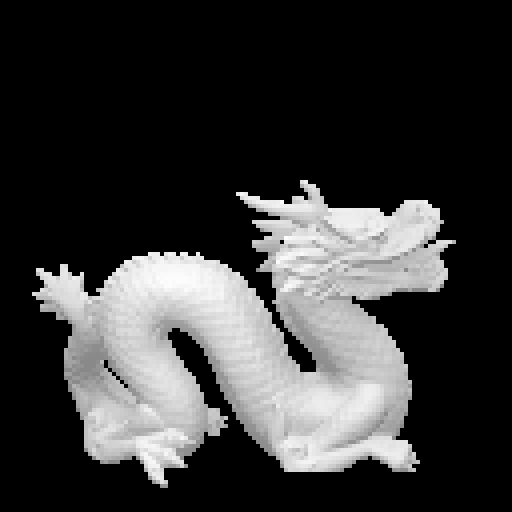
\includegraphics[width=\linewidth]{./Figures/visual_eval/fancy_eval_7_img.png}
		\caption{Image}
	\end{subfigure}
	\begin{subfigure}[b]{0.24\linewidth}
		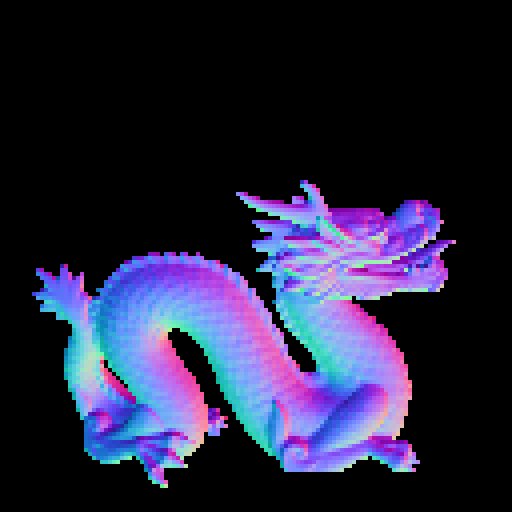
\includegraphics[width=\linewidth]{./Figures/visual_eval/fancy_eval_7_groundtruth.png}
		\caption{GT}
	\end{subfigure}
	\begin{subfigure}[b]{0.24\linewidth}
		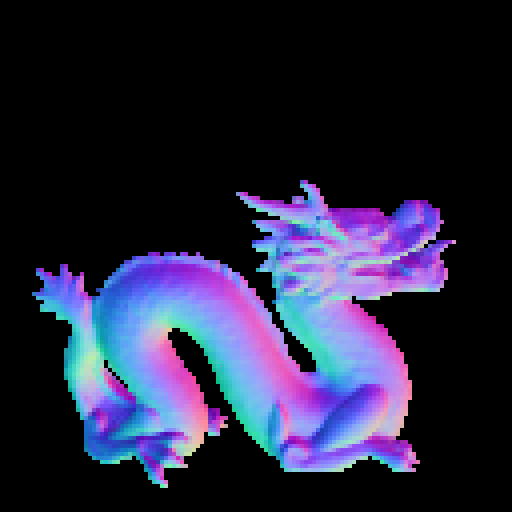
\includegraphics[width=\linewidth]{./Figures/visual_eval/fancy_eval_7_normal_GCNN-GCNN.png}
		\caption{Predict}
	\end{subfigure}
	\begin{subfigure}[b]{0.24\linewidth}
		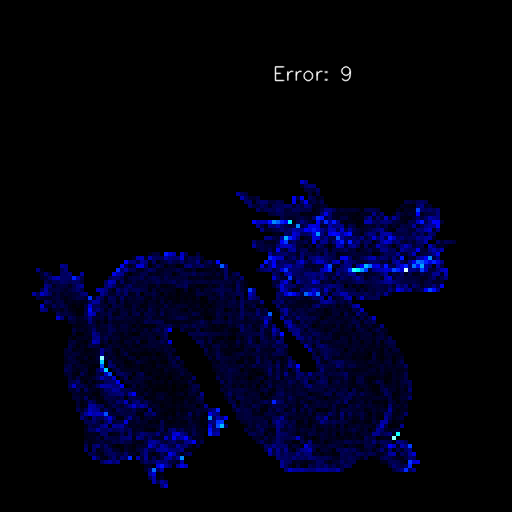
\includegraphics[width=\linewidth]{./Figures/visual_eval/fancy_eval_7_error_GCNN-GCNN.png}
		\caption{Error}
	\end{subfigure}
	
	\begin{tikzpicture}
		\node[text width=0.1\textwidth] at (10,-1) {90};
		\node[inner sep=0pt] (input) at (8,-1)
		{
\includegraphics[width=.2\textwidth]{./Figures/colorscale_blue.png}};
		\node[text width=0.3\textwidth] at (7,-1) {Error: 0};
	\end{tikzpicture}
	
	\caption{Normal inference based on GCNN. Test image has resolution $ 128\times128 $}
	\label{fig:gcnn-eval}
\end{figure}

%% GCNN zoom in eval
\begin{figure}[H]
	\centering
	\begin{subfigure}[b]{0.18\linewidth}
		\includegraphics[width=\linewidth]{./Figures/gcnn-synthetic/eval_7_22_-8_normal.png}
	\end{subfigure}
	\begin{subfigure}[b]{0.18\linewidth}
		\includegraphics[width=\linewidth]{./Figures/gcnn-synthetic/eval_7_2_22_normal.png}
	\end{subfigure}
	\begin{subfigure}[b]{0.18\linewidth}
		\includegraphics[width=\linewidth]{./Figures/gcnn-synthetic/eval_7_32_12_normal.png}
	\end{subfigure}
	\begin{subfigure}[b]{0.18\linewidth}
		\includegraphics[width=\linewidth]{./Figures/gcnn-synthetic/eval_7_42_-28_normal.png}
	\end{subfigure}
	\begin{subfigure}[b]{0.18\linewidth}
		\includegraphics[width=\linewidth]{./Figures/gcnn-synthetic/eval_7_12_-48_normal.png}
	\end{subfigure}
	
	\begin{subfigure}[b]{0.18\linewidth}
		\includegraphics[width=\linewidth]{./Figures/gcnn-synthetic/eval_7_22_-8_error.png}
		\caption{Scale}
	\end{subfigure}
	\begin{subfigure}[b]{0.18\linewidth}
		\includegraphics[width=\linewidth]{./Figures/gcnn-synthetic/eval_7_2_22_error.png}
		\caption{Head}
	\end{subfigure}
	\begin{subfigure}[b]{0.18\linewidth}
		\includegraphics[width=\linewidth]{./Figures/gcnn-synthetic/eval_7_32_12_error.png}
		\caption{Foreleg}
	\end{subfigure}
	\begin{subfigure}[b]{0.18\linewidth}
		\includegraphics[width=\linewidth]{./Figures/gcnn-synthetic/eval_7_42_-28_error.png}
		\caption{Hindleg}
	\end{subfigure}
	\begin{subfigure}[b]{0.18\linewidth}
		\includegraphics[width=\linewidth]{./Figures/gcnn-synthetic/eval_7_12_-48_error.png}
		\caption{Tail}
	\end{subfigure}
	
	
	\caption{Zoom in of some regions of Dragon object. The first row is surface normal, the second row is the corresponding errors. Zoom-in normal map corresponding $ 32\times32 $ points in the original matrix.}
	\label{fig:gcnn-eval-synthetic-zoom-in}
\end{figure}

%% compare to other models

%% GCNN zoom in eval
\begin{figure}[H]
	\centering
	\begin{subfigure}[b]{0.24\linewidth}
		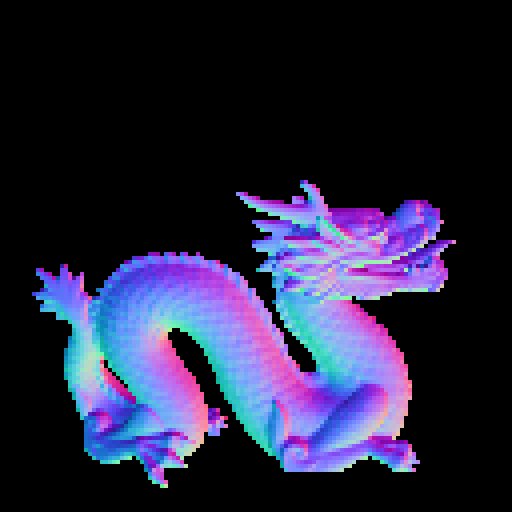
\includegraphics[width=\linewidth]{./Figures/visual_eval/fancy_eval_7_groundtruth.png}
	\end{subfigure}
	\begin{subfigure}[b]{0.24\linewidth}
		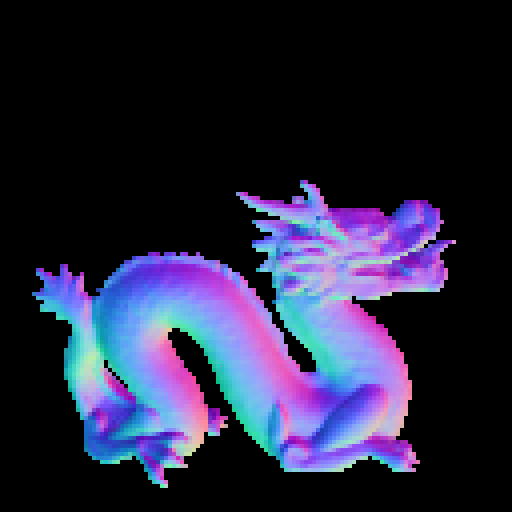
\includegraphics[width=\linewidth]{./Figures/visual_eval/fancy_eval_7_normal_GCNN-GCNN.png}
	\end{subfigure}
	\begin{subfigure}[b]{0.24\linewidth}
		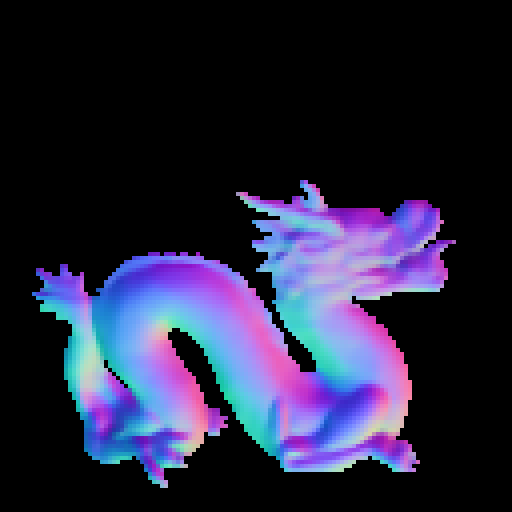
\includegraphics[width=\linewidth]{./Figures/visual_eval/fancy_eval_7_normal_GCNN-NOC.png}
	\end{subfigure}
	\begin{subfigure}[b]{0.24\linewidth}
		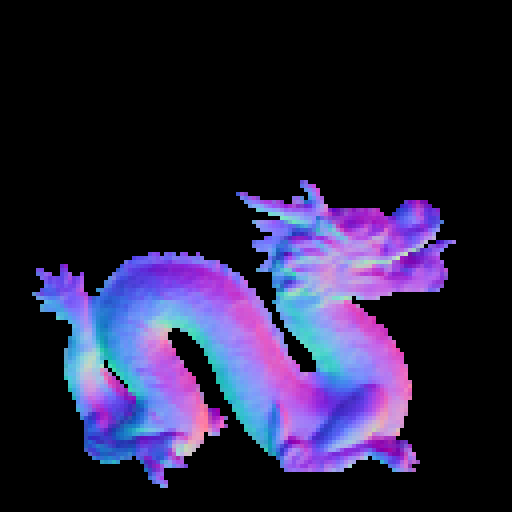
\includegraphics[width=\linewidth]{./Figures/visual_eval/fancy_eval_7_normal_GCNN-CNN.png}
	\end{subfigure}
	
	\begin{subfigure}[b]{0.24\linewidth}
		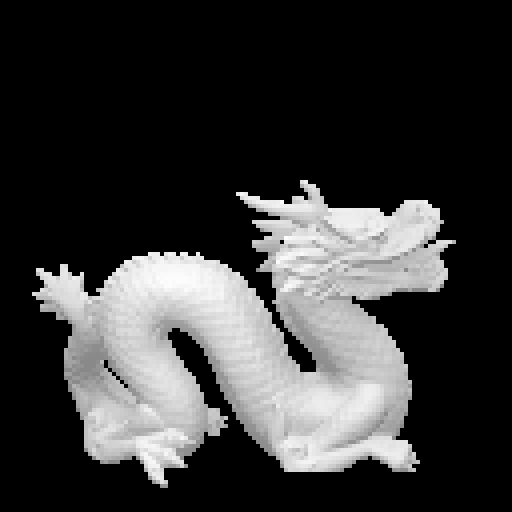
\includegraphics[width=\linewidth]{./Figures/visual_eval/fancy_eval_7_img.png}
		\caption{GT}
	\end{subfigure}
	\begin{subfigure}[b]{0.24\linewidth}
		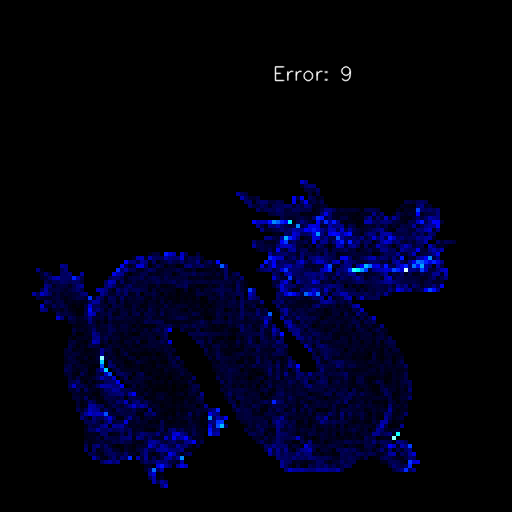
\includegraphics[width=\linewidth]{./Figures/visual_eval/fancy_eval_7_error_GCNN-GCNN.png}
		\caption{GCNN}
	\end{subfigure}
	\begin{subfigure}[b]{0.24\linewidth}
		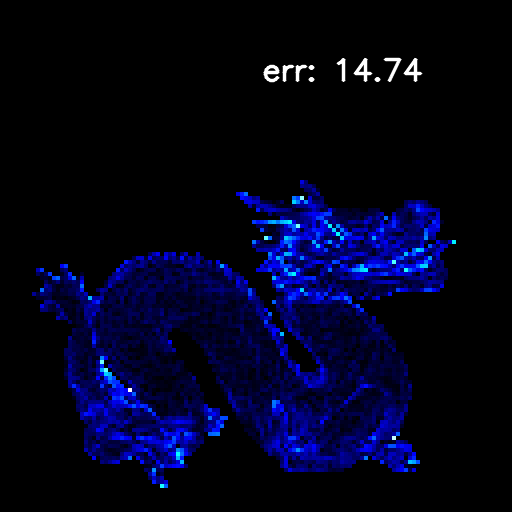
\includegraphics[width=\linewidth]{./Figures/visual_eval/fancy_eval_7_error_GCNN-NOC.png}
		\caption{NOC}
	\end{subfigure}
	\begin{subfigure}[b]{0.24\linewidth}
		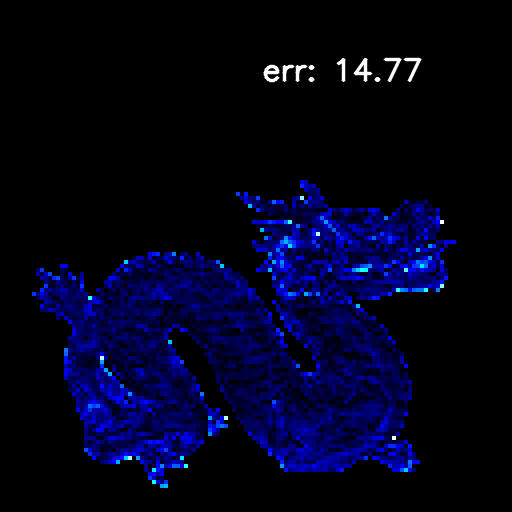
\includegraphics[width=\linewidth]{./Figures/visual_eval/fancy_eval_7_error_GCNN-CNN.png}
		\caption{CNN}
	\end{subfigure}
	
	
	\caption{Comparison of GCNN model with no skip connection version(NOC) and standard convolution layer only version (CNN). The second row is the corresponding mean average degree error.}
	\label{fig:gcnn-eval-multi-model}
\end{figure}



\newpage
\section{Visualized evaluation on Trip-Net models }

For the approach using illuminated calibrated RGBD image, the task is undertaken by Trip-Net introduced in \ref{sec:trip-net}. 
The qualitative evaluation is shown in figure \ref{fig:trip-eval}. In order to show the effectiveness of added illuminated information, the training settings for all the models are exact the same. We also use the same input as we did in GCNN evaluation. The error of Trip-Net is 6 degree whereas the GCNN is 9. 

As shown in the figure \ref{fig:tripnet-eval-synthetic-zoom-in}, the scale on the dragon body is much easier to detect and close to the ground-truth. The head region gives a sharper edge prediction. All of the five sampled zoom-in regions in the Trip-Net has a better performance than GCNN.

%% TripNet-eval
\begin{figure}[H]
	\centering
	\begin{subfigure}[b]{0.24\linewidth}
		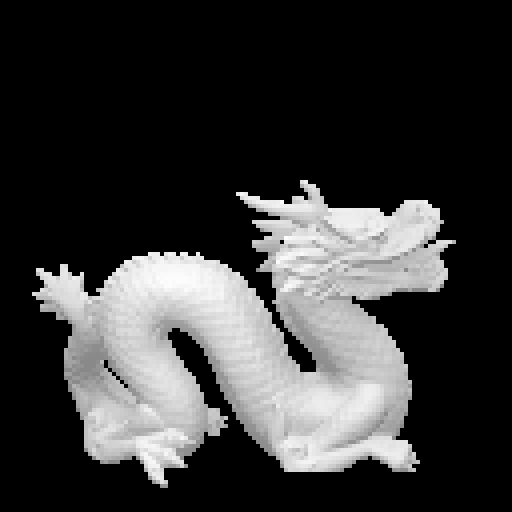
\includegraphics[width=\linewidth]{./Figures/visual_eval/fancy_eval_7_img.png}
		\caption{Image}
	\end{subfigure}
	\begin{subfigure}[b]{0.24\linewidth}
		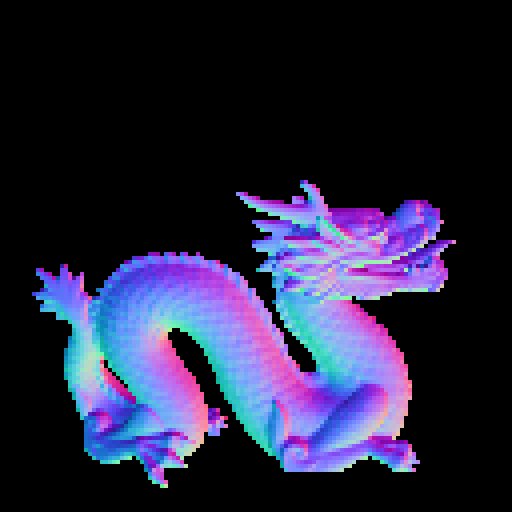
\includegraphics[width=\linewidth]{./Figures/visual_eval/fancy_eval_7_groundtruth.png}
		\caption{GT}
	\end{subfigure}
	\begin{subfigure}[b]{0.24\linewidth}
		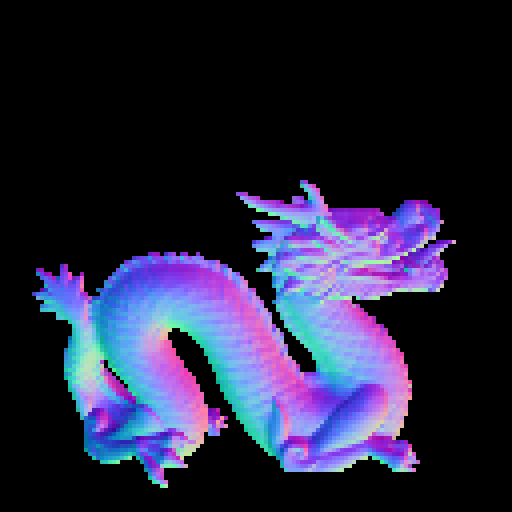
\includegraphics[width=\linewidth]{./Figures/visual_eval/fancy_eval_7_normal_an2-8-1000.png}
		\caption{Predict}
	\end{subfigure}
	\begin{subfigure}[b]{0.24\linewidth}
		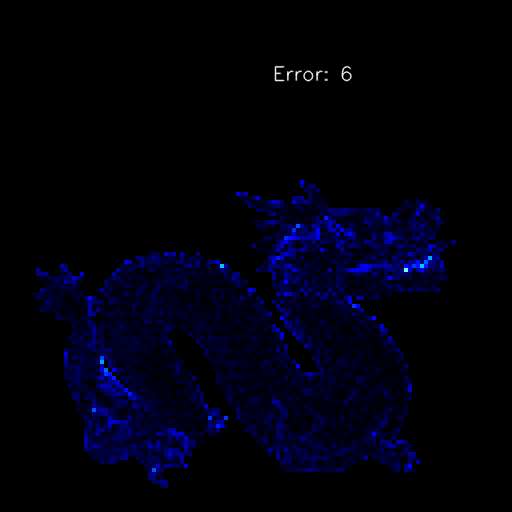
\includegraphics[width=\linewidth]{./Figures/visual_eval/fancy_eval_7_error_an2-8-1000.png}
		\caption{Error}
	\end{subfigure}
	
	\begin{tikzpicture}
		\node[text width=0.1\textwidth] at (10,-1) {90};
		\node[inner sep=0pt] (input) at (8,-1)
		{
\includegraphics[width=.2\textwidth]{./Figures/colorscale_blue.png}};
		\node[text width=0.3\textwidth] at (7,-1) {Error: 0};
	\end{tikzpicture}
	
	\caption{Normal inference based on Trip-Net. Test image has resolution $ 128\times128 $}
	\label{fig:trip-eval}
\end{figure}

%% tripNet zoom in eval
\begin{figure}[H]
	\centering
	\begin{subfigure}[b]{0.18\linewidth}
		\includegraphics[width=\linewidth]{./Figures/tripnet_synthetic/eval_7_22_-8_normal.png}
	\end{subfigure}
	\begin{subfigure}[b]{0.18\linewidth}
		\includegraphics[width=\linewidth]{./Figures/tripnet_synthetic/eval_7_2_22_normal.png}
	\end{subfigure}
	\begin{subfigure}[b]{0.18\linewidth}
		\includegraphics[width=\linewidth]{./Figures/tripnet_synthetic/eval_7_32_12_normal.png}
	\end{subfigure}
	\begin{subfigure}[b]{0.18\linewidth}
		\includegraphics[width=\linewidth]{./Figures/tripnet_synthetic/eval_7_42_-28_normal.png}
	\end{subfigure}
	\begin{subfigure}[b]{0.18\linewidth}
		\includegraphics[width=\linewidth]{./Figures/tripnet_synthetic/eval_7_12_-48_normal.png}
	\end{subfigure}
	
	\begin{subfigure}[b]{0.18\linewidth}
		\includegraphics[width=\linewidth]{./Figures/tripnet_synthetic/eval_7_22_-8_error.png}
		\caption{Scale}
	\end{subfigure}
	\begin{subfigure}[b]{0.18\linewidth}
		\includegraphics[width=\linewidth]{./Figures/tripnet_synthetic/eval_7_2_22_error.png}
		\caption{Head}
	\end{subfigure}
	\begin{subfigure}[b]{0.18\linewidth}
		\includegraphics[width=\linewidth]{./Figures/tripnet_synthetic/eval_7_32_12_error.png}
		\caption{Foreleg}
	\end{subfigure}
	\begin{subfigure}[b]{0.18\linewidth}
		\includegraphics[width=\linewidth]{./Figures/tripnet_synthetic/eval_7_42_-28_error.png}
		\caption{Hindleg}
	\end{subfigure}
	\begin{subfigure}[b]{0.18\linewidth}
		\includegraphics[width=\linewidth]{./Figures/tripnet_synthetic/eval_7_12_-48_error.png}
		\caption{Tail}
	\end{subfigure}
	
	
	\caption{Zoom in of some regions of Dragon object. The first row is surface normal, the second row is the corresponding errors. Zoom-in normal map corresponding $ 32\times32 $ points in the original matrix.}
	\label{fig:tripnet-eval-synthetic-zoom-in}
\end{figure}


%% F1-F4 eval

\begin{figure}[H]
	\centering
	\begin{subfigure}[b]{0.18\linewidth}
		\includegraphics[width=\linewidth]{./Figures/tripnet_synthetic/fancy_eval_7_groundtruth.png}
	\end{subfigure}
	\begin{subfigure}[b]{0.18\linewidth}
		\includegraphics[width=\linewidth]{./Figures/tripnet_synthetic/fancy_eval_7_normal_f1.png}
	\end{subfigure}
	\begin{subfigure}[b]{0.18\linewidth}
		\includegraphics[width=\linewidth]{./Figures/tripnet_synthetic/fancy_eval_7_normal_f2.png}
	\end{subfigure}
	\begin{subfigure}[b]{0.18\linewidth}
		\includegraphics[width=\linewidth]{./Figures/tripnet_synthetic/fancy_eval_7_normal_f3.png}
	\end{subfigure}
	\begin{subfigure}[b]{0.18\linewidth}
		\includegraphics[width=\linewidth]{./Figures/tripnet_synthetic/fancy_eval_7_normal_f4.png}
	\end{subfigure}
	
	
		\begin{subfigure}[b]{0.18\linewidth}
		\includegraphics[width=\linewidth]{./Figures/tripnet_synthetic/fancy_eval_7_img.png}
		\caption{GT}
	\end{subfigure}
	\begin{subfigure}[b]{0.18\linewidth}
		\includegraphics[width=\linewidth]{./Figures/tripnet_synthetic/fancy_eval_7_error_f1.png}
		\caption{F1}
	\end{subfigure}
	\begin{subfigure}[b]{0.18\linewidth}
		\includegraphics[width=\linewidth]{./Figures/tripnet_synthetic/fancy_eval_7_error_f2.png}
		\caption{F2}
	\end{subfigure}
	\begin{subfigure}[b]{0.18\linewidth}
		\includegraphics[width=\linewidth]{./Figures/tripnet_synthetic/fancy_eval_7_error_f3.png}
		\caption{F3}
	\end{subfigure}
	\begin{subfigure}[b]{0.18\linewidth}
		\includegraphics[width=\linewidth]{./Figures/tripnet_synthetic/fancy_eval_7_error_f4.png}
		\caption{F4}
	\end{subfigure}
	
	
	\caption{Comparison between different fusion times for Trip-Net. The first row is surface normal, the second row is the corresponding errors. The number in ``F$ x $" represents the fusion times. }
	\label{fig:tripnet-eval-synthetic-zoom-in}
\end{figure}



\section{More Comparison}
Figure \ref{fig:final-eval} gives more visualization on model SVD, GCNN and Trip-Net. Figure \ref{fig:final-eval-zoom-in} is the corresponding zoom-in visualization.
\newpage
%% Final-Visual
\begin{figure}
	\centering
	\begin{subfigure}[b]{0.24\linewidth}
		\includegraphics[width=\linewidth]{./Figures/visual_eval/fancy_eval_2_groundtruth.png}
	\end{subfigure}
	\begin{subfigure}[b]{0.24\linewidth}
		\includegraphics[width=\linewidth]{./Figures/visual_eval/fancy_eval_2_normal_an2-8-1000.png}
	\end{subfigure}
	\begin{subfigure}[b]{0.24\linewidth}
		\includegraphics[width=\linewidth]{./Figures/visual_eval/fancy_eval_2_normal_GCNN-GCNN.png}
	\end{subfigure}
	\begin{subfigure}[b]{0.24\linewidth}
		\includegraphics[width=\linewidth]{./Figures/visual_eval/fancy_eval_2_normal_SVD.png}
	\end{subfigure}
	
	\begin{subfigure}[b]{0.24\linewidth}
		\includegraphics[width=\linewidth]{./Figures/visual_eval/fancy_eval_2_img.png}
	\end{subfigure}
	\begin{subfigure}[b]{0.24\linewidth}
		\includegraphics[width=\linewidth]{./Figures/visual_eval/fancy_eval_2_error_an2-8-1000.png}
	\end{subfigure}
	\begin{subfigure}[b]{0.24\linewidth}
		\includegraphics[width=\linewidth]{./Figures/visual_eval/fancy_eval_2_error_GCNN-GCNN.png}
	\end{subfigure}
	\begin{subfigure}[b]{0.24\linewidth}
		\includegraphics[width=\linewidth]{./Figures/visual_eval/fancy_eval_2_error_SVD.png}
	\end{subfigure}
	
	\begin{subfigure}[b]{0.24\linewidth}
		\includegraphics[width=\linewidth]{./Figures/visual_eval/fancy_eval_3_groundtruth.png}
	\end{subfigure}
	\begin{subfigure}[b]{0.24\linewidth}
		\includegraphics[width=\linewidth]{./Figures/visual_eval/fancy_eval_3_normal_an2-8-1000.png}
	\end{subfigure}
	\begin{subfigure}[b]{0.24\linewidth}
		\includegraphics[width=\linewidth]{./Figures/visual_eval/fancy_eval_3_normal_GCNN-GCNN.png}
	\end{subfigure}
	\begin{subfigure}[b]{0.24\linewidth}
		\includegraphics[width=\linewidth]{./Figures/visual_eval/fancy_eval_3_normal_SVD.png}
	\end{subfigure}
	
	
	
	\begin{subfigure}[b]{0.24\linewidth}
		\includegraphics[width=\linewidth]{./Figures/visual_eval/fancy_eval_3_img.png}
	\end{subfigure}
	\begin{subfigure}[b]{0.24\linewidth}
		\includegraphics[width=\linewidth]{./Figures/visual_eval/fancy_eval_3_error_an2-8-1000.png}
	\end{subfigure}
	\begin{subfigure}[b]{0.24\linewidth}
		\includegraphics[width=\linewidth]{./Figures/visual_eval/fancy_eval_3_error_GCNN-GCNN.png}
	\end{subfigure}
	\begin{subfigure}[b]{0.24\linewidth}
		\includegraphics[width=\linewidth]{./Figures/visual_eval/fancy_eval_3_error_SVD.png}
	\end{subfigure}
	
	\begin{subfigure}[b]{0.24\linewidth}
		\includegraphics[width=\linewidth]{./Figures/visual_eval/fancy_eval_9_groundtruth.png}
	\end{subfigure}
	\begin{subfigure}[b]{0.24\linewidth}
		\includegraphics[width=\linewidth]{./Figures/visual_eval/fancy_eval_9_normal_an2-8-1000.png}
	\end{subfigure}
	\begin{subfigure}[b]{0.24\linewidth}
		\includegraphics[width=\linewidth]{./Figures/visual_eval/fancy_eval_9_normal_GCNN-GCNN.png}
	\end{subfigure}
	\begin{subfigure}[b]{0.24\linewidth}
		\includegraphics[width=\linewidth]{./Figures/visual_eval/fancy_eval_9_normal_SVD.png}
	\end{subfigure}
	
	
	\begin{subfigure}[b]{0.24\linewidth}
		\includegraphics[width=\linewidth]{./Figures/visual_eval/fancy_eval_9_img.png}
		\caption{GT}
	\end{subfigure}
	\begin{subfigure}[b]{0.24\linewidth}
		\includegraphics[width=\linewidth]{./Figures/visual_eval/fancy_eval_9_error_an2-8-1000.png}
		\caption{TripNet}
	\end{subfigure}
	\begin{subfigure}[b]{0.24\linewidth}
		\includegraphics[width=\linewidth]{./Figures/visual_eval/fancy_eval_9_error_GCNN-GCNN.png}
		\caption{GCNN}
	\end{subfigure}
	\begin{subfigure}[b]{0.24\linewidth}
		\includegraphics[width=\linewidth]{./Figures/visual_eval/fancy_eval_9_error_SVD.png}
		\caption{SVD}
	\end{subfigure}
	
	
	\begin{tikzpicture}
		\node[text width=0.1\textwidth] at (10,-1) {90};
		\node[inner sep=0pt] (input) at (8,-1)
		{\includegraphics[width=.2\textwidth]{./Figures/colorscale_blue.png}};
		\node[text width=0.3\textwidth] at (7,-1) {Error: 0};
	\end{tikzpicture}
	
	\caption{Evaluation on objects Baoshanlu, Washington statue, Bus(from top to bottom).}
	\label{fig:final-eval}
\end{figure}


%% Final-Visual-Zoom-In
\begin{figure}
	\centering
	\begin{subfigure}[b]{0.24\linewidth}
		\includegraphics[width=\linewidth]{./Figures/visual_eval/eval_2_normal_GT.png}
	\end{subfigure}
	\begin{subfigure}[b]{0.24\linewidth}
		\includegraphics[width=\linewidth]{./Figures/visual_eval/eval_2_normal_an2-8-1000.png}
	\end{subfigure}
	\begin{subfigure}[b]{0.24\linewidth}
		\includegraphics[width=\linewidth]{./Figures/visual_eval/eval_2_normal_GCNN-GCNN.png}
	\end{subfigure}
	\begin{subfigure}[b]{0.24\linewidth}
		\includegraphics[width=\linewidth]{./Figures/visual_eval/eval_2_normal_SVD.png}
	\end{subfigure}
	
	\begin{subfigure}[b]{0.24\linewidth}
		\includegraphics[width=\linewidth]{./Figures/visual_eval/eval_2_img.png}
	\end{subfigure}
	\begin{subfigure}[b]{0.24\linewidth}
		\includegraphics[width=\linewidth]{./Figures/visual_eval/eval_2_error_an2-8-1000.png}
	\end{subfigure}
	\begin{subfigure}[b]{0.24\linewidth}
		\includegraphics[width=\linewidth]{./Figures/visual_eval/eval_2_error_GCNN-GCNN.png}
	\end{subfigure}
	\begin{subfigure}[b]{0.24\linewidth}
		\includegraphics[width=\linewidth]{./Figures/visual_eval/eval_2_error_SVD.png}
	\end{subfigure}
	
	
	
	
	\begin{subfigure}[b]{0.24\linewidth}
		\includegraphics[width=\linewidth]{./Figures/visual_eval/eval_3_normal_GT.png}
	\end{subfigure}
	\begin{subfigure}[b]{0.24\linewidth}
		\includegraphics[width=\linewidth]{./Figures/visual_eval/eval_3_normal_an2-8-1000.png}
	\end{subfigure}
	\begin{subfigure}[b]{0.24\linewidth}
		\includegraphics[width=\linewidth]{./Figures/visual_eval/eval_3_normal_GCNN-GCNN.png}
	\end{subfigure}
	\begin{subfigure}[b]{0.24\linewidth}
		\includegraphics[width=\linewidth]{./Figures/visual_eval/eval_3_normal_SVD.png}
	\end{subfigure}
	
	\begin{subfigure}[b]{0.24\linewidth}
		\includegraphics[width=\linewidth]{./Figures/visual_eval/eval_3_img.png}
	\end{subfigure}
	\begin{subfigure}[b]{0.24\linewidth}
		\includegraphics[width=\linewidth]{./Figures/visual_eval/eval_3_error_an2-8-1000.png}
	\end{subfigure}
	\begin{subfigure}[b]{0.24\linewidth}
		\includegraphics[width=\linewidth]{./Figures/visual_eval/eval_3_error_GCNN-GCNN.png}
	\end{subfigure}
	\begin{subfigure}[b]{0.24\linewidth}
		\includegraphics[width=\linewidth]{./Figures/visual_eval/eval_3_error_SVD.png}
	\end{subfigure}
	
	
	
	\begin{subfigure}[b]{0.24\linewidth}
		\includegraphics[width=\linewidth]{./Figures/visual_eval/eval_9_normal_GT.png}
	\end{subfigure}
	\begin{subfigure}[b]{0.24\linewidth}
		\includegraphics[width=\linewidth]{./Figures/visual_eval/eval_9_normal_an2-8-1000.png}
	\end{subfigure}
	\begin{subfigure}[b]{0.24\linewidth}
		\includegraphics[width=\linewidth]{./Figures/visual_eval/eval_9_normal_GCNN-GCNN.png}
	\end{subfigure}
	\begin{subfigure}[b]{0.24\linewidth}
		\includegraphics[width=\linewidth]{./Figures/visual_eval/eval_9_normal_SVD.png}
	\end{subfigure}
	
	
	\begin{subfigure}[b]{0.24\linewidth}
		\includegraphics[width=\linewidth]{./Figures/visual_eval/eval_9_img.png}
		\caption{GT}
	\end{subfigure}
	\begin{subfigure}[b]{0.24\linewidth}
		\includegraphics[width=\linewidth]{./Figures/visual_eval/eval_9_error_an2-8-1000.png}
		\caption{Trip-Net}
	\end{subfigure}
	\begin{subfigure}[b]{0.24\linewidth}
		\includegraphics[width=\linewidth]{./Figures/visual_eval/eval_9_error_GCNN-GCNN.png}
		\caption{GCNN}
	\end{subfigure}
	\begin{subfigure}[b]{0.24\linewidth}
		\includegraphics[width=\linewidth]{./Figures/visual_eval/eval_9_error_SVD.png}
		\caption{SVD}
	\end{subfigure}
	
	\caption{Zoom in of the center region of the objects in Figure \ref{fig:final-eval}}
	\label{fig:final-eval-zoom-in}
\end{figure}


\section{Trining on higher resolution}
We also prepared the dataset with resolution $ 512\times 512 $ for model evaluation. Higher resolution gives more information about the surface feature using the same model compare to lower resolution. The benefit is, if we extract a fixed sized patch from the normal map, say $ 32 \times 32 $, it might correspond a hindleg area of the dragon object in $ 128\times 128 $ resolution but maybe only a toe in $ 512\times 512 $ resolution. Therefore if we still use the same kernel size in the network for the same dataset, the higher the resolution it has, the less area it will cover. This is a good thing. Because then we only need to use these $ 32\times 32 $ points to calculate a toe in $ 512\times512 $ resolution image. But in $ 128\times128 $ resolution image, we use the same area $ 32\times32 $ to calculate the whole hindleg. In another word, we can also say that the higher resolution ``smooth" the object surface. Thus the higher resolution helps the model to calculate a more accurate normal map. 

We use the same settings and the same models for training work on dataset with $ 512\times512 $ resolution. Figure \ref{fig:high_resolution_eval} gives a comparison among SVD, GCNN and Trip-Net models.



\begin{figure}[H]
	\centering
	\begin{subfigure}[b]{0.24\linewidth}
		\includegraphics[width=\linewidth]{./Figures/comparison/fancy_eval_22_groundtruth.png}
	\end{subfigure}
	\begin{subfigure}[b]{0.24\linewidth}
		\includegraphics[width=\linewidth]{./Figures/comparison/fancy_eval_22_normal_SVD.png}
	\end{subfigure}
	\begin{subfigure}[b]{0.24\linewidth}
		\includegraphics[width=\linewidth]{./Figures/comparison/fancy_eval_22_normal_GCNN-512.png}
	\end{subfigure}
	\begin{subfigure}[b]{0.24\linewidth}
		\includegraphics[width=\linewidth]{./Figures/comparison/fancy_eval_14_normal_Trip-Net-512.png}
	\end{subfigure}
	
	
	\begin{subfigure}[b]{0.24\linewidth}
		\includegraphics[width=\linewidth]{./Figures/comparison/fancy_eval_22_img.png}
		\caption{GT}
	\end{subfigure}
	\begin{subfigure}[b]{0.24\linewidth}
		\includegraphics[width=\linewidth]{./Figures/comparison/fancy_eval_22_error_SVD.png}
		\caption{SVD}
	\end{subfigure}
	\begin{subfigure}[b]{0.24\linewidth}
		\includegraphics[width=\linewidth]{./Figures/comparison/fancy_eval_22_error_GCNN-512.png}
		\caption{GCNN}
	\end{subfigure}
	\begin{subfigure}[b]{0.24\linewidth}
		\includegraphics[width=\linewidth]{./Figures/comparison/fancy_eval_14_error_Trip-Net-512.png}
		\caption{Trip-Net}
	\end{subfigure}

	
	
	\caption{Comparison between different SVD, GCNN and Trip-Net model on $ 512\times 512 $ dataset. The first row is surface normal, the second row is the corresponding errors. }
	\label{fig:high_resolution_eval}
\end{figure}

%% 5 degree metric
\begin{table}[H]
	\centering
	\begin{tabular}{l l l l }
		\tabhead{Metrics} & \tabhead{SVD} & \tabhead{GCNN} & \tabhead{Trip-Net} \\
		Mean  					& 8.88 & 5.82 & 5.72 \\ 
		\hline
		Median					& 3.66 & 3.98 & 3.99 \\ 
		\hline
		$ 5^\circ $ 			& 0.63 & 0.63 & 0.62 \\
		\hline
		$ 11.5^\circ $ 			& 0.79 & 0.89 & 0.90 \\
		\hline
		$ 22.5^\circ $ 			& 0.89 & 0.97 & 0.97 \\
		\hline
		$ 30^\circ $ 			& 0.92 & 0.98 & 0.99 \\
	\end{tabular}
	\caption{Evaluation of SVD, GCNN and Trip-Net models on 6 different metrics based on 100 test scenes.}	
	\label{tab:high_resolution_eval}
\end{table}


\section{Training on Real-Dataset}


\begin{figure}[H]
	\centering
	\begin{subfigure}[b]{0.24\linewidth}
		\includegraphics[width=\linewidth]{./Figures/comparison/fancy_eval_14_groundtruth.png}
	\end{subfigure}
	\begin{subfigure}[b]{0.24\linewidth}
		\includegraphics[width=\linewidth]{./Figures/comparison/fancy_eval_14_normal_SVD.png}
	\end{subfigure}
	\begin{subfigure}[b]{0.24\linewidth}
		\includegraphics[width=\linewidth]{./Figures/comparison/fancy_eval_14_normal_GCNN-512-269.png}
	\end{subfigure}
	\begin{subfigure}[b]{0.24\linewidth}
		\includegraphics[width=\linewidth]{./Figures/comparison/fancy_eval_14_normal_Trip-Net-512.png}
	\end{subfigure}
	
	
	\begin{subfigure}[b]{0.24\linewidth}
		\includegraphics[width=\linewidth]{./Figures/comparison/fancy_eval_14_img.png}
		\caption{GT}
	\end{subfigure}
	\begin{subfigure}[b]{0.24\linewidth}
		\includegraphics[width=\linewidth]{./Figures/comparison/fancy_eval_14_error_SVD.png}
		\caption{SVD}
	\end{subfigure}
	\begin{subfigure}[b]{0.24\linewidth}
		\includegraphics[width=\linewidth]{./Figures/comparison/fancy_eval_14_error_GCNN-512-269.png}
		\caption{GCNN}
	\end{subfigure}
	\begin{subfigure}[b]{0.24\linewidth}
		\includegraphics[width=\linewidth]{./Figures/comparison/fancy_eval_14_error_Trip-Net-512.png}
		\caption{Trip-Net}
	\end{subfigure}
	
	
	
	\caption{Comparison between different SVD, GCNN and Trip-Net model on $ 512\times 512 $ dataset. The first row is surface normal, the second row is the corresponding errors. }
	\label{fig:high_resolution_eval}
\end{figure}

\begin{table}[H]
	\centering
	\begin{tabular}{l l l l }
		\tabhead{Metrics} & \tabhead{SVD} & \tabhead{GCNN} & \tabhead{Trip-Net} \\
		Mean  					& 8.20 & 8.90 & 8.80\\ 
		\hline
		Median					& 4.87 & 5.82 & 5.66 \\ 
		\hline
		$ 5^\circ $ 			& 0.51 & 0.43 & 0.44 \\
		\hline
		$ 11.5^\circ $ 			& 0.79 & 0.78 & 0.78 \\
		\hline
		$ 22.5^\circ $ 			& 0.93 & 0.93 & 0.93 \\
		\hline
		$ 30^\circ $ 			& 0.96 & 0.96 & 0.96\\
	\end{tabular}
	\caption{Evaluation of SVD, GCNN and Trip-Net models on 6 different metrics based on 100 test scenes.}	
	\label{tab:high_resolution_eval}
\end{table}


\end{document}
